\documentclass[a4paper,12pt]{article}
\usepackage{amsmath, amsthm, amssymb, geometry}
\usepackage{xcolor}
\usepackage{float}
\usepackage{pgf,tikz}
\usepackage[pdfinfo=on]{xepersian}
\settextfont{XB Niloofar}
\setlatintextfont{Times New Roman}

\geometry{margin=2.5cm}
\linespread{1.2}

\newtheoremstyle{exercise}{3pt}{3pt}{\normalfont}{}{\bfseries}{\\}{0pt}{}
\theoremstyle{exercise}
\newtheorem{exercise}{تمرین}
\newtheorem{solution}{پاسخ}
\renewcommand{\theexercise}{}
\renewcommand{\thesolution}{}

\title{%
	\Huge \textbf{تمرین} \\[0.3cm]
	\Large حسابان - مقدمه
}
\author{علی عاشوری}
\date{\today}

\begin{document}
	
	\maketitle
	
	\section*{وضعیت}
	\begin{itemize}
		\item \textbf{درس:} حسابان (حساب دیفرانسیل و انتگرال)
		\item \textbf{فصل:} مقدمه (مقدمه‌ای بر انتگرال)
		\item \textbf{شماره‌ی تمرین:} ۱
		\item \textbf{تاریخ حل:} \lr{July 12, 2026}
		\item \textbf{وضعیت:} \textcolor{blue}{حل‌شده}
		\item \textbf{منبع:} \lr{Calculus 1, Tom Apostol.}
	\end{itemize}
	\rule{\textwidth}{0.4pt}
	
	\begin{exercise}
		مساحت زیر نمودار
		$x^3$
		از
		$x=0$
		تا
		$x=b$
		را با روش ارشمیدس به دست آورید.
	\end{exercise}
	
	\bigskip
	
	\begin{solution}
		نمودار تابع
		$x^3$
		را در نظر بگیرید. اگر سطح زیر نمودار را با تعداد $n$ مستطیل بپوشانیم، دو حالت به وجود می‌آید. حالت اول این است که نقاط روی نمودار، نقاط سمت راست مستطیل‌ها هستند و حالت دوم این است که نقاط روی نمودار، نقاط سمت چپ مستطیل‌ها هستند. برای مثال، دو شکل زیر را ببینید که این کار با تعداد $6$ مستطیل انجام شده است.
		\begin{center}
			% Right Endpoints Used
			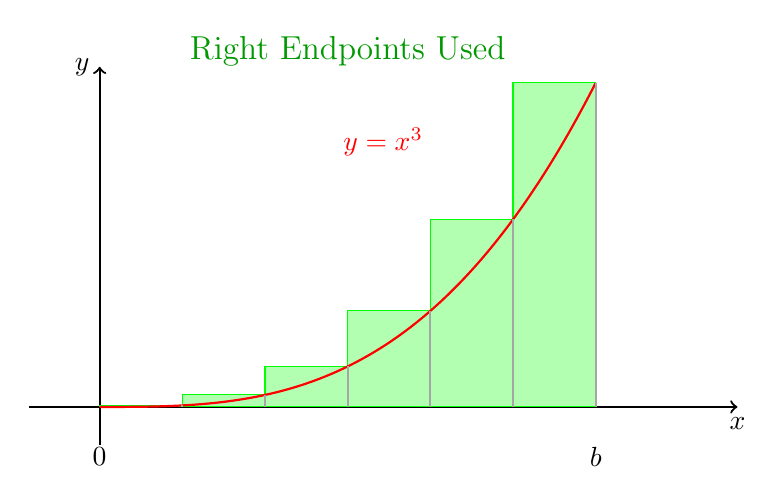
\begin{tikzpicture}[scale=1.2, x=1.5cm, y=0.08cm]
				\def\b{3.5}
				\def\n{6}
				\pgfmathsetmacro{\h}{\b/\n}
				
				\draw[->,thick] (-0.5,0) -- (4.5,0) node[below] {$x$};
				\draw[->,thick] (0,-5) -- (0,45) node[left] {$y$};
				
				\foreach \i in {0,...,\n} {
					\pgfmathsetmacro{\xLeft}{\i*\h}
					\pgfmathsetmacro{\xRight}{(\i+1)*\h}
					\ifnum \i<\n
					\pgfmathsetmacro{\yRight}{\xRight*\xRight*\xRight}
					\draw[fill=green!30, draw=green] (\xLeft,0) rectangle (\xRight,\yRight);
					\fi
				}
				
				\draw[red, thick, smooth, samples=100, domain=0:\b] plot(\x, {\x*\x*\x});
				\node at (0, -15pt) {$0$};
				\node at (\b, -15pt) {$b$};
				\node at (2, 35) [red] {$y = x^3$};
				
				\foreach \i in {0,...,\n} {
					\pgfmathsetmacro{\xPoint}{\i*\h}
					\draw[gray!70, thick] (\xPoint,0) -- (\xPoint, {\xPoint*\xPoint*\xPoint});
				}
				\node at (1.75, 47) [green!60!black, font=\large] {Right Endpoints Used};
			\end{tikzpicture}
			
			\bigskip
			
			% Left Endpoints Used
			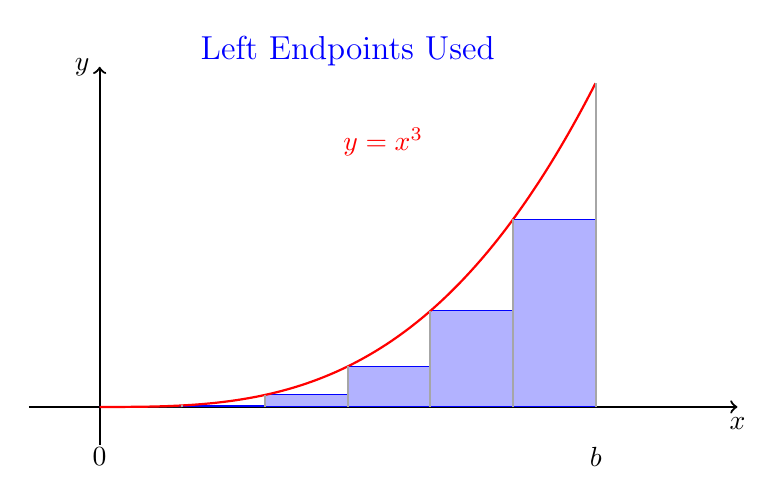
\begin{tikzpicture}[scale=1.2, x=1.5cm, y=0.08cm]
				\def\b{3.5}
				\def\n{6}
				\pgfmathsetmacro{\h}{\b/\n}
				
				\draw[->,thick] (-0.5,0) -- (4.5,0) node[below] {$x$};
				\draw[->,thick] (0,-5) -- (0,45) node[left] {$y$};
				
				\foreach \i in {0,...,\n} {
					\pgfmathsetmacro{\xLeft}{\i*\h}
					\pgfmathsetmacro{\xRight}{(\i+1)*\h}
					\ifnum \i<\n
					\pgfmathsetmacro{\yLeft}{\xLeft*\xLeft*\xLeft}
					\draw[fill=blue!30, draw=blue] (\xLeft,0) rectangle (\xRight,\yLeft);
					\fi
				}
				
				\draw[red, thick, smooth, samples=100, domain=0:\b] plot(\x, {\x*\x*\x});
				\node at (0, -15pt) {$0$};
				\node at (\b, -15pt) {$b$};
				\node at (2, 35) [red] {$y = x^3$};
				
				\foreach \i in {0,...,\n} {
					\pgfmathsetmacro{\xPoint}{\i*\h}
					\draw[gray!70, thick] (\xPoint,0) -- (\xPoint, {\xPoint*\xPoint*\xPoint});
				}
				\node at (1.75, 47) [blue, font=\large] {Left Endpoints Used};
			\end{tikzpicture}
		\end{center}
		
		حال فرض کنید که همین کار با $n$ مستطیل انجام شود که $n$ یک عدد طبیعی است. واضح است که به ازای هر عدد طبیعی $n$، مساحت زیر نمودار بین مساحت حالت اول و دوم است. به عبارت دیگر، از مساحت حالت اول کوچکتر و از مساحت حالت دوم بزرگتر است. مساحت حالت اول (مستطیل‌های بالای نمودار) را
		$S(n)$
		, مساحت حالت دوم (مستطیل‌های زیر نمودار) را
		$s(n)$
		می‌نامیم. به دو شکل زیر نگاه کنید.
		
		\begin{center}
			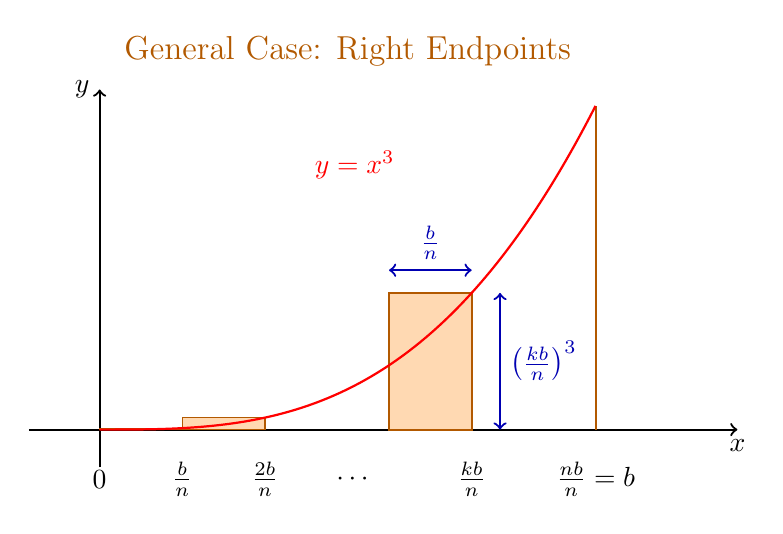
\begin{tikzpicture}[scale=1.2, x=1.5cm, y=0.08cm]
			\def\b{3.5}
			\def\n{6}
			\pgfmathsetmacro{\h}{\b/\n}
			
			\draw[->,thick] (-0.5,0) -- (4.5,0) node[below] {$x$};
			\draw[->,thick] (0,-5) -- (0,45) node[left] {$y$};
			
			% مستطیل اول
			\pgfmathsetmacro{\xRightOne}{\h}
			\pgfmathsetmacro{\yRightOne}{\xRightOne*\xRightOne*\xRightOne}
			\draw[fill=orange!30, draw=orange!70!black] (0,0) rectangle (\xRightOne,\yRightOne);
			\draw[orange!70!black, thick] (\xRightOne,0) -- (\xRightOne,\yRightOne);
			\node at (\xRightOne, -15pt) {$\frac{b}{n}$};
			
			% مستطیل دوم
			\pgfmathsetmacro{\xRightTwo}{2*\h}
			\pgfmathsetmacro{\yRightTwo}{\xRightTwo*\xRightTwo*\xRightTwo}
			\draw[fill=orange!30, draw=orange!70!black] (\h,0) rectangle (\xRightTwo,\yRightTwo);
			\draw[orange!70!black, thick] (\xRightTwo,0) -- (\xRightTwo,\yRightTwo);
			\node at (\xRightTwo, -15pt) {$\frac{2b}{n}$};
			
			\node at (1.8, -15pt) {$\cdots$};
			
			% مستطیل وسط
			\pgfmathsetmacro{\k}{4.5}
			\pgfmathsetmacro{\xRightK}{\k*\h}
			\pgfmathsetmacro{\xLeftK}{(\k-1)*\h}
			\pgfmathsetmacro{\yRightK}{\xRightK*\xRightK*\xRightK}
			
			\draw[fill=orange!30, draw=orange!70!black, thick] 
			(\xLeftK,0) rectangle (\xRightK,\yRightK);
			\draw[orange!70!black, thick] (\xRightK,0) -- (\xRightK,\yRightK);
			
			% فلش طول در بالای مستطیل
			\draw[<->, thick, blue!70!black] 
			(\xLeftK, \yRightK+3) -- (\xRightK, \yRightK+3) 
			node[midway, above] {$\frac{b}{n}$};
			
			% فلش عرض در سمت راست مستطیل
			\draw[<->, thick, blue!70!black] 
			(\xRightK+0.2, 0) -- (\xRightK+0.2, \yRightK) 
			node[midway, right] {$\left(\frac{kb}{n}\right)^3$};
			
			\node at (\xRightK, -15pt) {$\frac{kb}{n}$};
			
			% خط مرز سمت راست
			\pgfmathsetmacro{\yRightLast}{\b*\b*\b}
			\draw[orange!70!black, thick] (\b,0) -- (\b,\yRightLast);
			\node at (\b, -15pt) {$\frac{nb}{n}=b$};
			
			\draw[red, thick, smooth, samples=100, domain=0:\b] plot(\x, {\x*\x*\x});
			\node at (0, -15pt) {$0$};
			\node at (1.8, 35) [red] {$y = x^3$};
			\node at (1.75, 50) [orange!70!black, font=\large] {General Case: Right Endpoints};
			\end{tikzpicture}
			
			\bigskip
			
				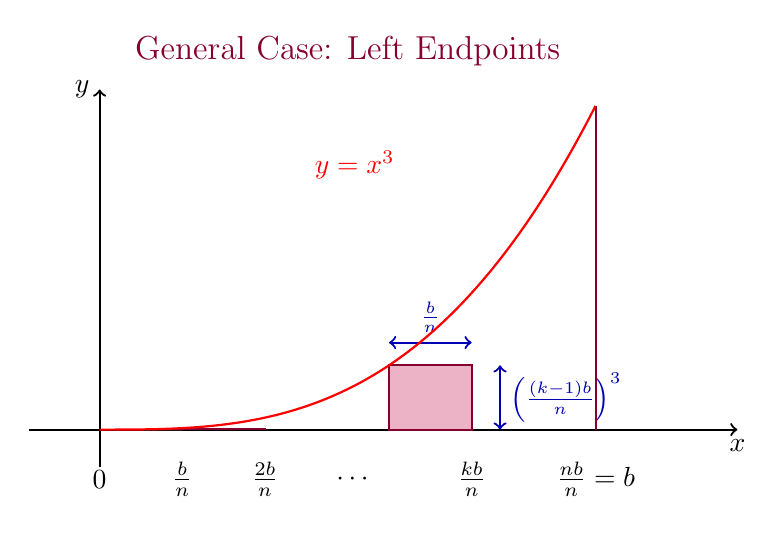
\begin{tikzpicture}[scale=1.2, x=1.5cm, y=0.08cm]
				\def\b{3.5}
				\def\n{6}
				\pgfmathsetmacro{\h}{\b/\n}
				
				\draw[->,thick] (-0.5,0) -- (4.5,0) node[below] {$x$};
				\draw[->,thick] (0,-5) -- (0,45) node[left] {$y$};
				
				% مستطیل اول (نقطه چپ = 0)
				\pgfmathsetmacro{\xRightOne}{\h}
				\pgfmathsetmacro{\yLeftOne}{0}
				\draw[fill=purple!30, draw=purple!70!black] (0,0) rectangle (\xRightOne,\yLeftOne);
				\draw[purple!70!black, thick] (\xRightOne,0) -- (\xRightOne,\yLeftOne);
				\node at (\xRightOne, -15pt) {$\frac{b}{n}$};
				
				% مستطیل دوم (نقطه چپ = b/n)
				\pgfmathsetmacro{\xRightTwo}{2*\h}
				\pgfmathsetmacro{\yLeftTwo}{\h*\h*\h}
				\draw[fill=purple!30, draw=purple!70!black] (\h,0) rectangle (\xRightTwo,\yLeftTwo);
				\draw[purple!70!black, thick] (\xRightTwo,0) -- (\xRightTwo,\yLeftTwo);
				\node at (\xRightTwo, -15pt) {$\frac{2b}{n}$};
				
				\node at (1.8, -15pt) {$\cdots$};
				
				% مستطیل وسط (نقطه چپ = (k-1)b/n)
				\pgfmathsetmacro{\k}{4.5}
				\pgfmathsetmacro{\xRightK}{\k*\h}
				\pgfmathsetmacro{\xLeftK}{(\k-1)*\h}
				\pgfmathsetmacro{\yLeftK}{\xLeftK*\xLeftK*\xLeftK}
				
				\draw[fill=purple!30, draw=purple!70!black, thick] 
				(\xLeftK,0) rectangle (\xRightK,\yLeftK);
				\draw[purple!70!black, thick] (\xRightK,0) -- (\xRightK,\yLeftK);
				
				% فلش طول در بالای مستطیل (کوچک‌تر)
				\draw[<->, thick, blue!70!black, font=\small] 
				(\xLeftK, \yLeftK+3) -- (\xRightK, \yLeftK+3) 
				node[midway, above] {$\frac{b}{n}$};
				
				% فلش عرض در سمت راست مستطیل (کوچک‌تر)
				\draw[<->, thick, blue!70!black, font=\small] 
				(\xRightK+0.2, 0) -- (\xRightK+0.2, \yLeftK) 
				node[midway, right] {$\left(\frac{(k-1)b}{n}\right)^3$};
				
				\node at (\xRightK, -15pt) {$\frac{kb}{n}$};
				
				% خط مرز سمت راست
				\pgfmathsetmacro{\yRightLast}{\b*\b*\b}
				\draw[purple!70!black, thick] (\b,0) -- (\b,\yRightLast);
				\node at (\b, -15pt) {$\frac{nb}{n}=b$};
				
				\draw[red, thick, smooth, samples=100, domain=0:\b] plot(\x, {\x*\x*\x});
				\node at (0, -15pt) {$0$};
				\node at (1.8, 35) [red] {$y = x^3$};
				\node at (1.75, 50) [purple!70!black, font=\large] {General Case: Left Endpoints};
			\end{tikzpicture}
		\end{center}
		
		ابتدا
		$S(n)$
		را به دست می‌آوریم. همان‌طور که در شکل نیز مشخص است، مساحت هر مستطیل برابر خواهد بود با:
		$$\left( \frac{b}{n} \right) \left( \frac{kb}{n} \right)^3$$
		که $k$ از $1$ تا $n$ تغییر می‌کند. بنابراین:
		$$S(n) = \sum_{k=1}^{n} \left( \frac{b}{n} \right) \left( \frac{kb}{n} \right)^3 = \sum_{k=1}^{n} \frac{k^3 b^4}{n^4}$$
		$$S(n)=\frac{b^4}{n^4} \left( 1^3 + 2^3 + \dots + n^3 \right)$$
		\\
		به روش مشابه،
		$s(n)$
		را به دست می‌آوریم.
		$$s(n) = \sum_{k=1}^{n} \frac{(k-1)^3 b^4}{n^4}$$
		$$s(n)=\frac{b^4}{n^4} \left( 1^3 + 2^3 + \dots + (n-1)^3 \right)$$
		\\
		اکنون سعی می‌کنیم مقداری بین
		$S(n)$ و $s(n)$
		بیابیم. اتحاد زیر را در نظر بگیرید.
		$$(k+1)^3 - k^3 = 3k^2 + 3k + 1$$
		برای هر $k$ از $1$ تا
		$n-1$
		این اتحاد را بازنویسی می‌کنیم.
		$$2^3 - 1^3 = 3 \cdot 1^2 + 3 \cdot 1 + 1$$
		$$3^3 - 2^3 = 3 \cdot 2^2 + 3 \cdot 2 + 1$$
		$$\vdots$$
		$$n^3 - (n-1)^3 = 3(n-1)^2 + 3(n-1) + 1$$
		در بالا، تعداد
		$n-1$
		تساوی داریم. طرف‌های چپ را با هم و طرف‌های راست را با هم جمع می‌کنیم.
		$$n^3 - 1 = 3 \left( 1^2 + 2^2 + \dots + (n-1)^2 \right) + 3 \left( 1 + 2 + \dots + (n-1) \right) + (n-1)$$
		می‌دانیم که (به راحتی اثبات می‌شود، در نتیجه اینجا اثبات نکرده‌ایم):
		$$1 + 2 + \dots + (n-1) = \frac{n(n-1)}{2}$$
		بنابراین می‌توانیم بنویسیم:
		$$1^2 + 2^2 + \dots + (n-1)^2 = \frac{n^3}{3} - \frac{n(n-1)}{2} + \frac{n}{3}$$
		$$1^2 + 2^2 + \dots + (n-1)^2 = \frac{2n^3 - 3n^2 + n}{6}$$
		\\
		اکنون اتحاد زیر را در نظر بگیرید.
		$$(k+1)^4 - k^4 = 4k^3 + 6k^2 + 4k + 1$$
		برای هر $k$ از $1$ تا
		$n-1$
		این اتحاد را بازنویسی می‌کنیم.
		$$2^4 - 1^4 = 4 \cdot 1^3 + 6 \cdot 1^2 + 4 \cdot 1 + 1$$
		$$3^4 - 2^4 = 4 \cdot 2^3 + 6 \cdot 2^2 + 4 \cdot 2 + 1$$
		$$\vdots$$
		$$n^4 - (n-1)^4 = 4(n-1)^3 + 6(n-1)^2 + 4(n-1) + 1$$
		در بالا، تعداد
		$n-1$
		تساوی داریم. طرف‌های چپ را با هم و طرف‌های راست را با هم جمع می‌کنیم.
		$$n^4 - 1 = 4 \left( 1^3 + 2^3 + \dots + (n-1)^3 \right) + 6 \left( 1^2 + 2^2 + \dots + (n-1)^2 \right) + 4 \left( 1 + 2 + \dots + (n-1) \right) + (n-1)$$
		$$n^4 = 4 \left( 1^3 + 2^3 + \dots + (n-1)^3 \right) + 6 \left( \frac{2n^3 - 3n^2 + n}{6} \right) + 4 \left( \frac{n(n-1)}{2} \right) + n$$
		بنابراین خواهیم داشت:
		$$1^3 + 2^3 + \dots + (n-1)^3 = \frac{n^4}{4} - \frac{2n^3 - n^2}{4}$$
		ادعا می‌کنیم که:
		$$1^3 + 2^3 + \dots + (n-1)^3 < \frac{n^4}{4}$$
		و برای اثبات این ادعا کافی است نشان دهیم که:
		$$\frac{2n^3 - n^2}{4} > 0 \ \Leftrightarrow \ 2n-1 > 0 \ \Leftrightarrow \ n > \frac{1}{2}$$
		توجه کنید که $n$ عددی صحیح و مثبت است.
		\\
		\\
		اکنون تساوی زیر را در نظر بگیرید.
		$$1^3 + 2^3 + \dots + (n-1)^3 + n^3= \frac{n^4}{4} - \frac{2n^3 - n^2}{4} + n^3$$
		$$1^3 + 2^3 + \dots + n^3= \frac{n^4}{4} + \frac{2n^3 + n^2}{4}$$
		ادعا می‌کنیم که:
		$$1^3 + 2^3 + \dots + n^3 > \frac{n^4}{4}$$
		و برای اثبات این ادعا کافی است نشان دهیم که:
		$$\frac{2n^3 + n^2}{4} > 0 \ \Leftrightarrow \ 2n+1 > 0 \ \Leftrightarrow \ n > -\frac{1}{2}$$
		توجه کنید که $n$ عددی صحیح و مثبت است.
		\\
		\\
		حال دو نامساوی به‌دست‌آمده را با هم در نظر بگیرید. توجه کنید که این دو نامساوی به ازای هر عدد صحیح مثبت $n$ برقرار است.
		$$1^3 + 2^3 + \dots + (n-1)^3 < \frac{n^4}{4} < 1^3 + 2^3 + \dots + n^3$$
		$$\frac{b^4}{n^4} \left( 1^3 + 2^3 + \dots + (n-1)^3 \right) < \frac{b^4}{4} < \frac{b^4}{n^4} \left( 1^3 + 2^3 + \dots + n^3 \right)$$
		$$s(n) < \frac{b^4}{4} < S(n)$$
		توانستیم مقداری بین $s(n)$ و $S(n)$ به دست آوریم. یادآوری می‌شود که مساحت ناحیه‌ی مشخص‌شده زیر نمودار، به ازای هر عدد صحیح مثبت $n$ باید بین $s(n)$ و $S(n)$ باشد. اما هنوز نمی‌توانیم ادعا کنیم که این مقدار برابر
		$\frac{b^4}{4}$
		است. لازم است نشان دهیم که هیچ عدد دیگری در نامساوی بالا صدق نمی‌کند. فرض کنید عدد دیگری به نام $A$ در نامساوی بالا صدق کند. در این صورت خواهیم داشت:
		$$s(n) < A, \frac{b^4}{4} < S(n)$$
		واضح است که اختلاف
		$\frac{b^4}{4}$
		و $A$ باید کوچکتر از اختلاف $s(n)$ و $S(n)$ باشد.
		$$\left| \frac{b^4}{4} - A \right| < S(n) - s(n)$$
		$$\left| \frac{b^4}{4} - A \right| < \frac{b^4}{n^4}(n^3)$$
		$$\left| \frac{b^4}{4} - A \right| < \frac{b^4}{n}$$
		$$n < \frac{b^4}{\left| \frac{b^4}{4} - A \right|}$$
		اما واضح است که نامساوی بالا به ازای هر عدد صحیح مثبت $n$ برقرار نیست. در نتیجه، فرض غلط است و $A$ نمی‌تواند بین $s(n)$ و $S(n)$ باشد، مگر اینکه $A$ همان
		$\frac{b^4}{4}$
		باشد. بنابراین
		$\frac{b^4}{4}$
		جوابی یکتا است.
		
		بنابراین، توانستیم مساحت زیر نمودار
		$x^3$
		از
		$x=0$
		تا
		$x=b$
		را به دست آوریم که برابر با مقدار $\frac{b^4}{4}$ است.
		\qed
	\end{solution}
	
	\section*{یادداشت‌ها}
	\begin{itemize}
		\item
		در کتاب \lr{Apostol} محاسبه‌ی مساحت زیر نمودار سهمی آورده شده است. به روش مشابه، می‌توان این کار را برای نمودار
		$x^n$
		به ازای هر $n$ طبیعی انجام داد. برای این کار باید نامساوی $s(n) < \frac{b^n}{n} < S(n)$ را در حالت کلی ثابت کرد. احتمالاً بعداً این کار را انجام دهم.
		\item 
		در کتاب \lr{Apostol} به روش دیگری ثابت کرده است که مقدار بین $s(n)$ و $S(n)$ یکتا است. راه‌حل من کوتاه‌تر است و به نظر درست می‌آید.
	\end{itemize}
	
\end{document}
